\documentclass[compress]{beamer}
\usepackage{ifthen,verbatim}

\newcommand{\isnote}{}
\xdefinecolor{lightyellow}{rgb}{1.,1.,0.25}
\xdefinecolor{darkblue}{rgb}{0.1,0.1,0.7}
\xdefinecolor{darkgreen}{rgb}{0.,0.5,0.}

%% Uncomment this to get annotations
%% \def\notes{\addtocounter{page}{-1}
%%            \renewcommand{\isnote}{*}
%% 	   \beamertemplateshadingbackground{lightyellow}{white}
%%            \begin{frame}
%%            \frametitle{Notes for the previous page (page \insertpagenumber)}
%%            \itemize}
%% \def\endnotes{\enditemize
%% 	      \end{frame}
%%               \beamertemplateshadingbackground{white}{white}
%%               \renewcommand{\isnote}{}}

%% Uncomment this to not get annotations
\def\notes{\comment}
\def\endnotes{\endcomment}

\setbeamertemplate{navigation symbols}{}
\setbeamertemplate{headline}{\mbox{ } \hfill
\begin{minipage}{5.5 cm}
\vspace{-0.75 cm} \small
\end{minipage} \hfill
\begin{minipage}{4.5 cm}
\vspace{-0.75 cm} \small
\begin{flushright}
\ifthenelse{\equal{\insertpagenumber}{1}}{}{Jim Pivarski \hspace{0.2 cm} \insertpagenumber\isnote/\pageref{numpages}}
\end{flushright}
\end{minipage}\mbox{\hspace{0.2 cm}}\includegraphics[height=1 cm]{../cmslogo} \hspace{0.1 cm} \includegraphics[height=1 cm]{../tamulogo} \hspace{0.01 cm} \vspace{-1.05 cm}}

\newcommand{\s}[1]{{\mbox{\scriptsize #1}}}

\begin{document}
\begin{frame}
\vfill
\begin{center}
\textcolor{darkblue}{\Large Testing barrel twist with beam-halo \& transfer lines}

\vfill
\begin{columns}
\column{0.3\linewidth}
\begin{center}
\large
Jim Pivarski
\end{center}
\end{columns}

\begin{columns}
\column{0.3\linewidth}
\begin{center}
\scriptsize
{\it Texas A\&M University}
\end{center}
\end{columns}

\vfill
24 September, 2010

\end{center}
\end{frame}

%% \begin{notes}
%% \item This is the annotated version of my talk.
%% \item If you want the version that I am presenting, download the one
%% labeled ``slides'' on Indico (or just ignore these yellow pages).
%% \item The annotated version is provided for extra detail and a written
%% record of comments that I intend to make orally.
%% \item Yellow notes refer to the content on the {\it previous} page.
%% \item All other slides are identical for the two versions.
%% \end{notes}

\small

\begin{frame}
\frametitle{Motivation}
\begin{itemize}
\item Barrel hardware and track-based methods yield almost the same
  geometry (RMS 1.3~mm) up to a systematic twist (4~mm)
\item Attempts to check each system for errors only strengthened the contradiction:
\end{itemize}

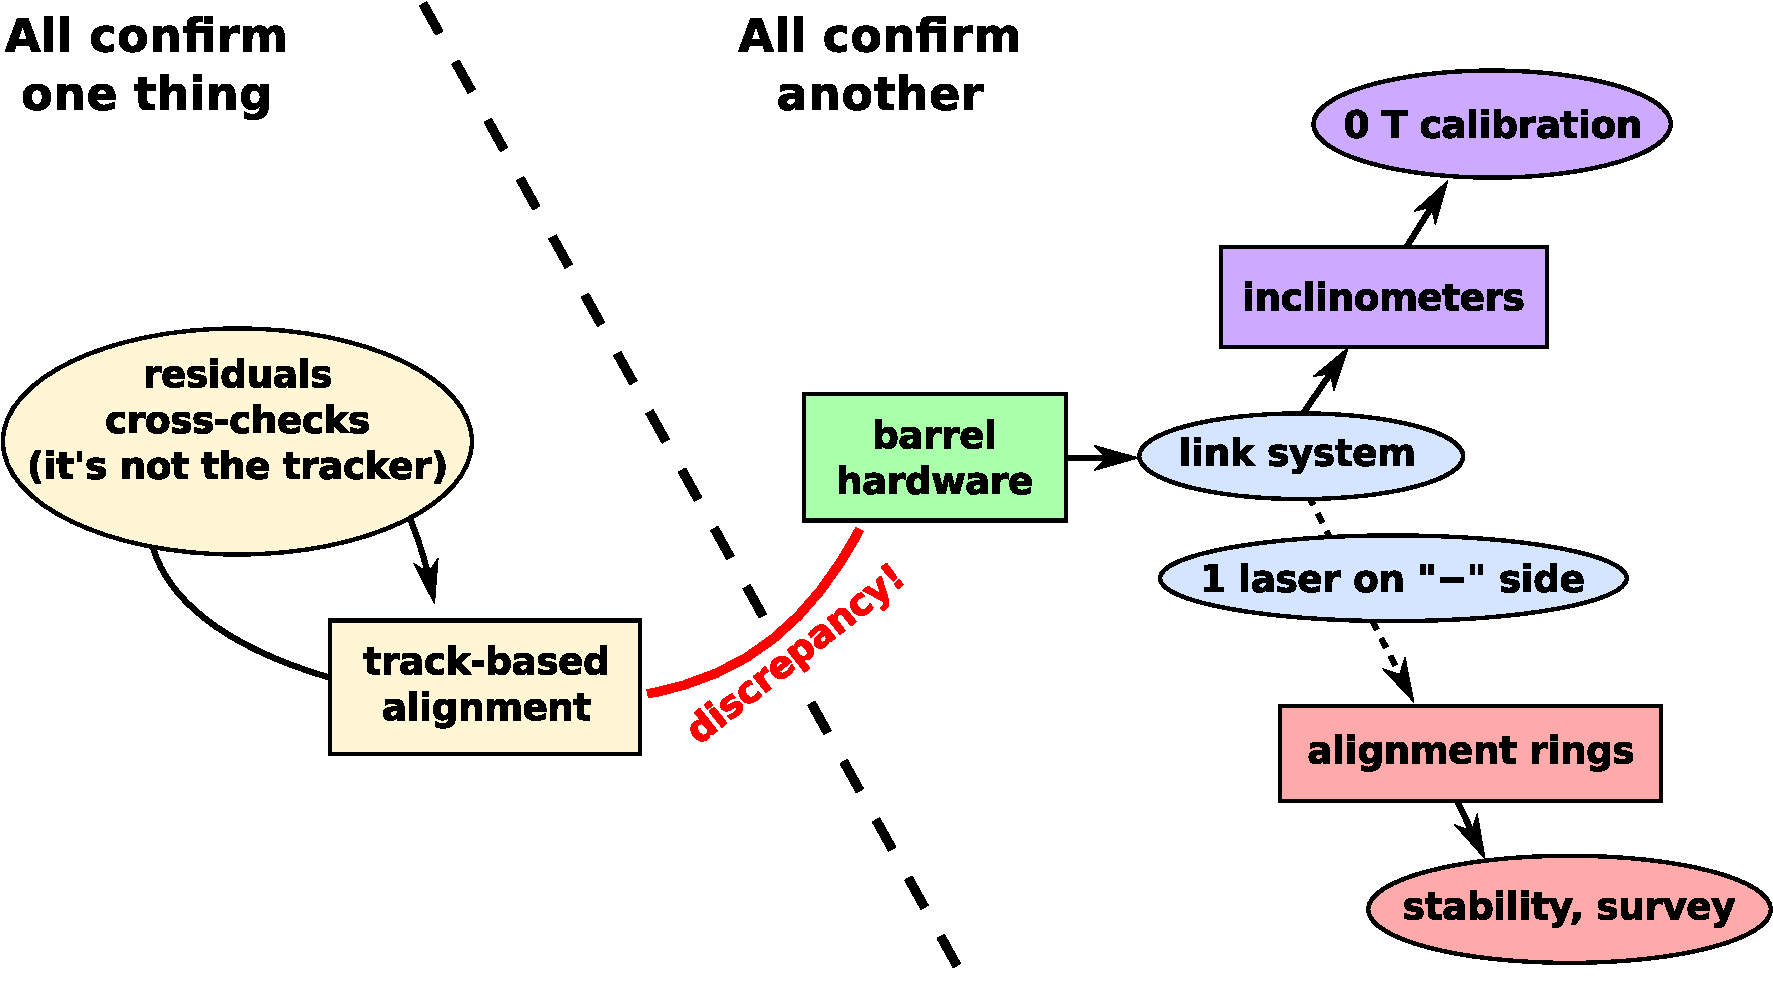
\includegraphics[width=\linewidth]{separate.pdf}
%% \hspace{-0.83 cm} \textcolor{darkblue}{\Large Outline2}
\end{frame}

\begin{frame}
\frametitle{Motivation}
\begin{itemize}\setlength{\itemsep}{0.3 cm}
\item The problem is that this isn't conclusive enough to tell us
  what to do next: we continue to look at our own systems for a sign
  of a problem while suspecting that it really lies in the
  other system

\item \textcolor{darkblue}{We need a method with a tighter network of
  cross-checks, more checks between hardware and tracks, and a larger
  number of degrees of freedom}

\item Any use of CSC hits, rather than just DT, would be good because
  detector problems are not likely to be the same

\item Any use of local tracks, rather than just global, would also be
  good, because this is a global effect
\end{itemize}
\end{frame}

\begin{frame}
\frametitle{Idea \#1: DT-CSC overlap}
\begin{columns}
\column{0.35\linewidth}
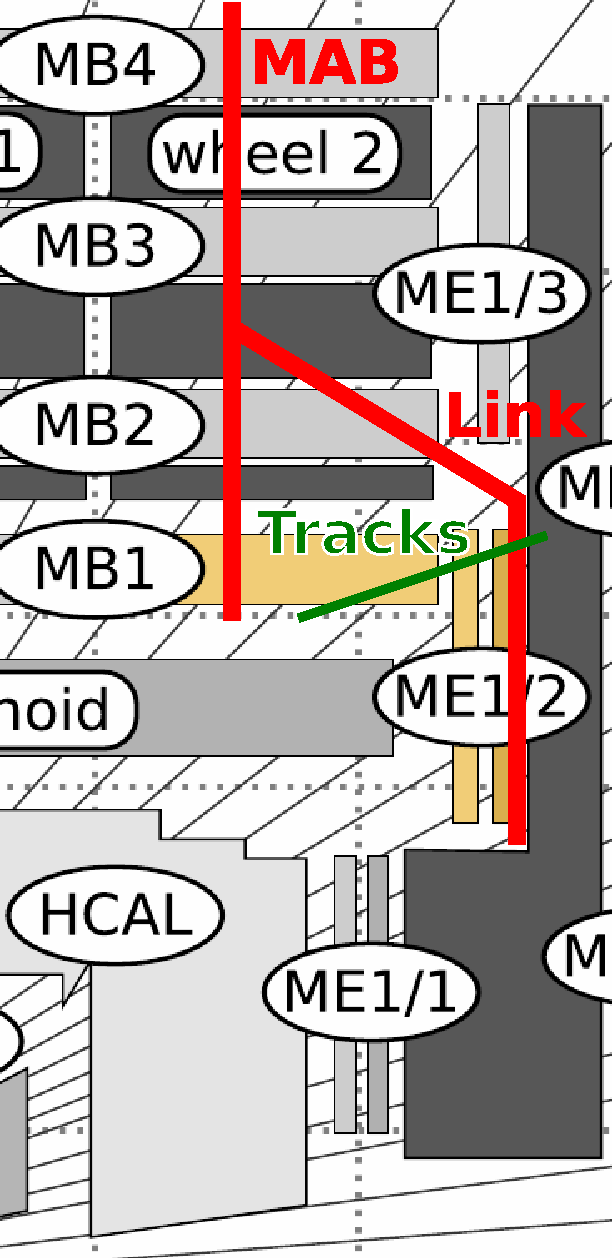
\includegraphics[width=\linewidth]{overlap_region.pdf}

\column{0.65\linewidth}
\begin{itemize}
\item \textcolor{darkblue}{Idea:} use Link system or transfer lines to
  put wheel $+$2 and ME$+$1 in the same coordinate system; look for kinks in
  tracks or at least discontinuities in residuals distributions across
  the border

\item \textcolor{darkblue}{If tracks/residuals are smooth:} then we
  will know that there are no local track reconstruction issues {\bf and}
  that the Link system is working well

\item \textcolor{darkblue}{If not:} then one of the two is broken

\item \textcolor{darkblue}{But in neither case do we learn if the
  barrel is twisted}

\item It's a good study to do, and should be done at some point
\end{itemize}

\begin{minipage}{\linewidth}
\tiny Complications: (1) CSC chamber positions must be prepared as a
CSCAlignmentRcd for track-reconstruction (2) only monitored CSCs can
be trusted, which reduces track statistics, (3) the magnetic field is
significantly radial in this region: calibration and field-map are
important, (4) there aren't many cosmic rays in this region; need to
use collisions
\end{minipage}
\end{columns}
\end{frame}

\begin{frame}
\frametitle{Idea \#2: beam-halo/transfer lines}
\begin{center}
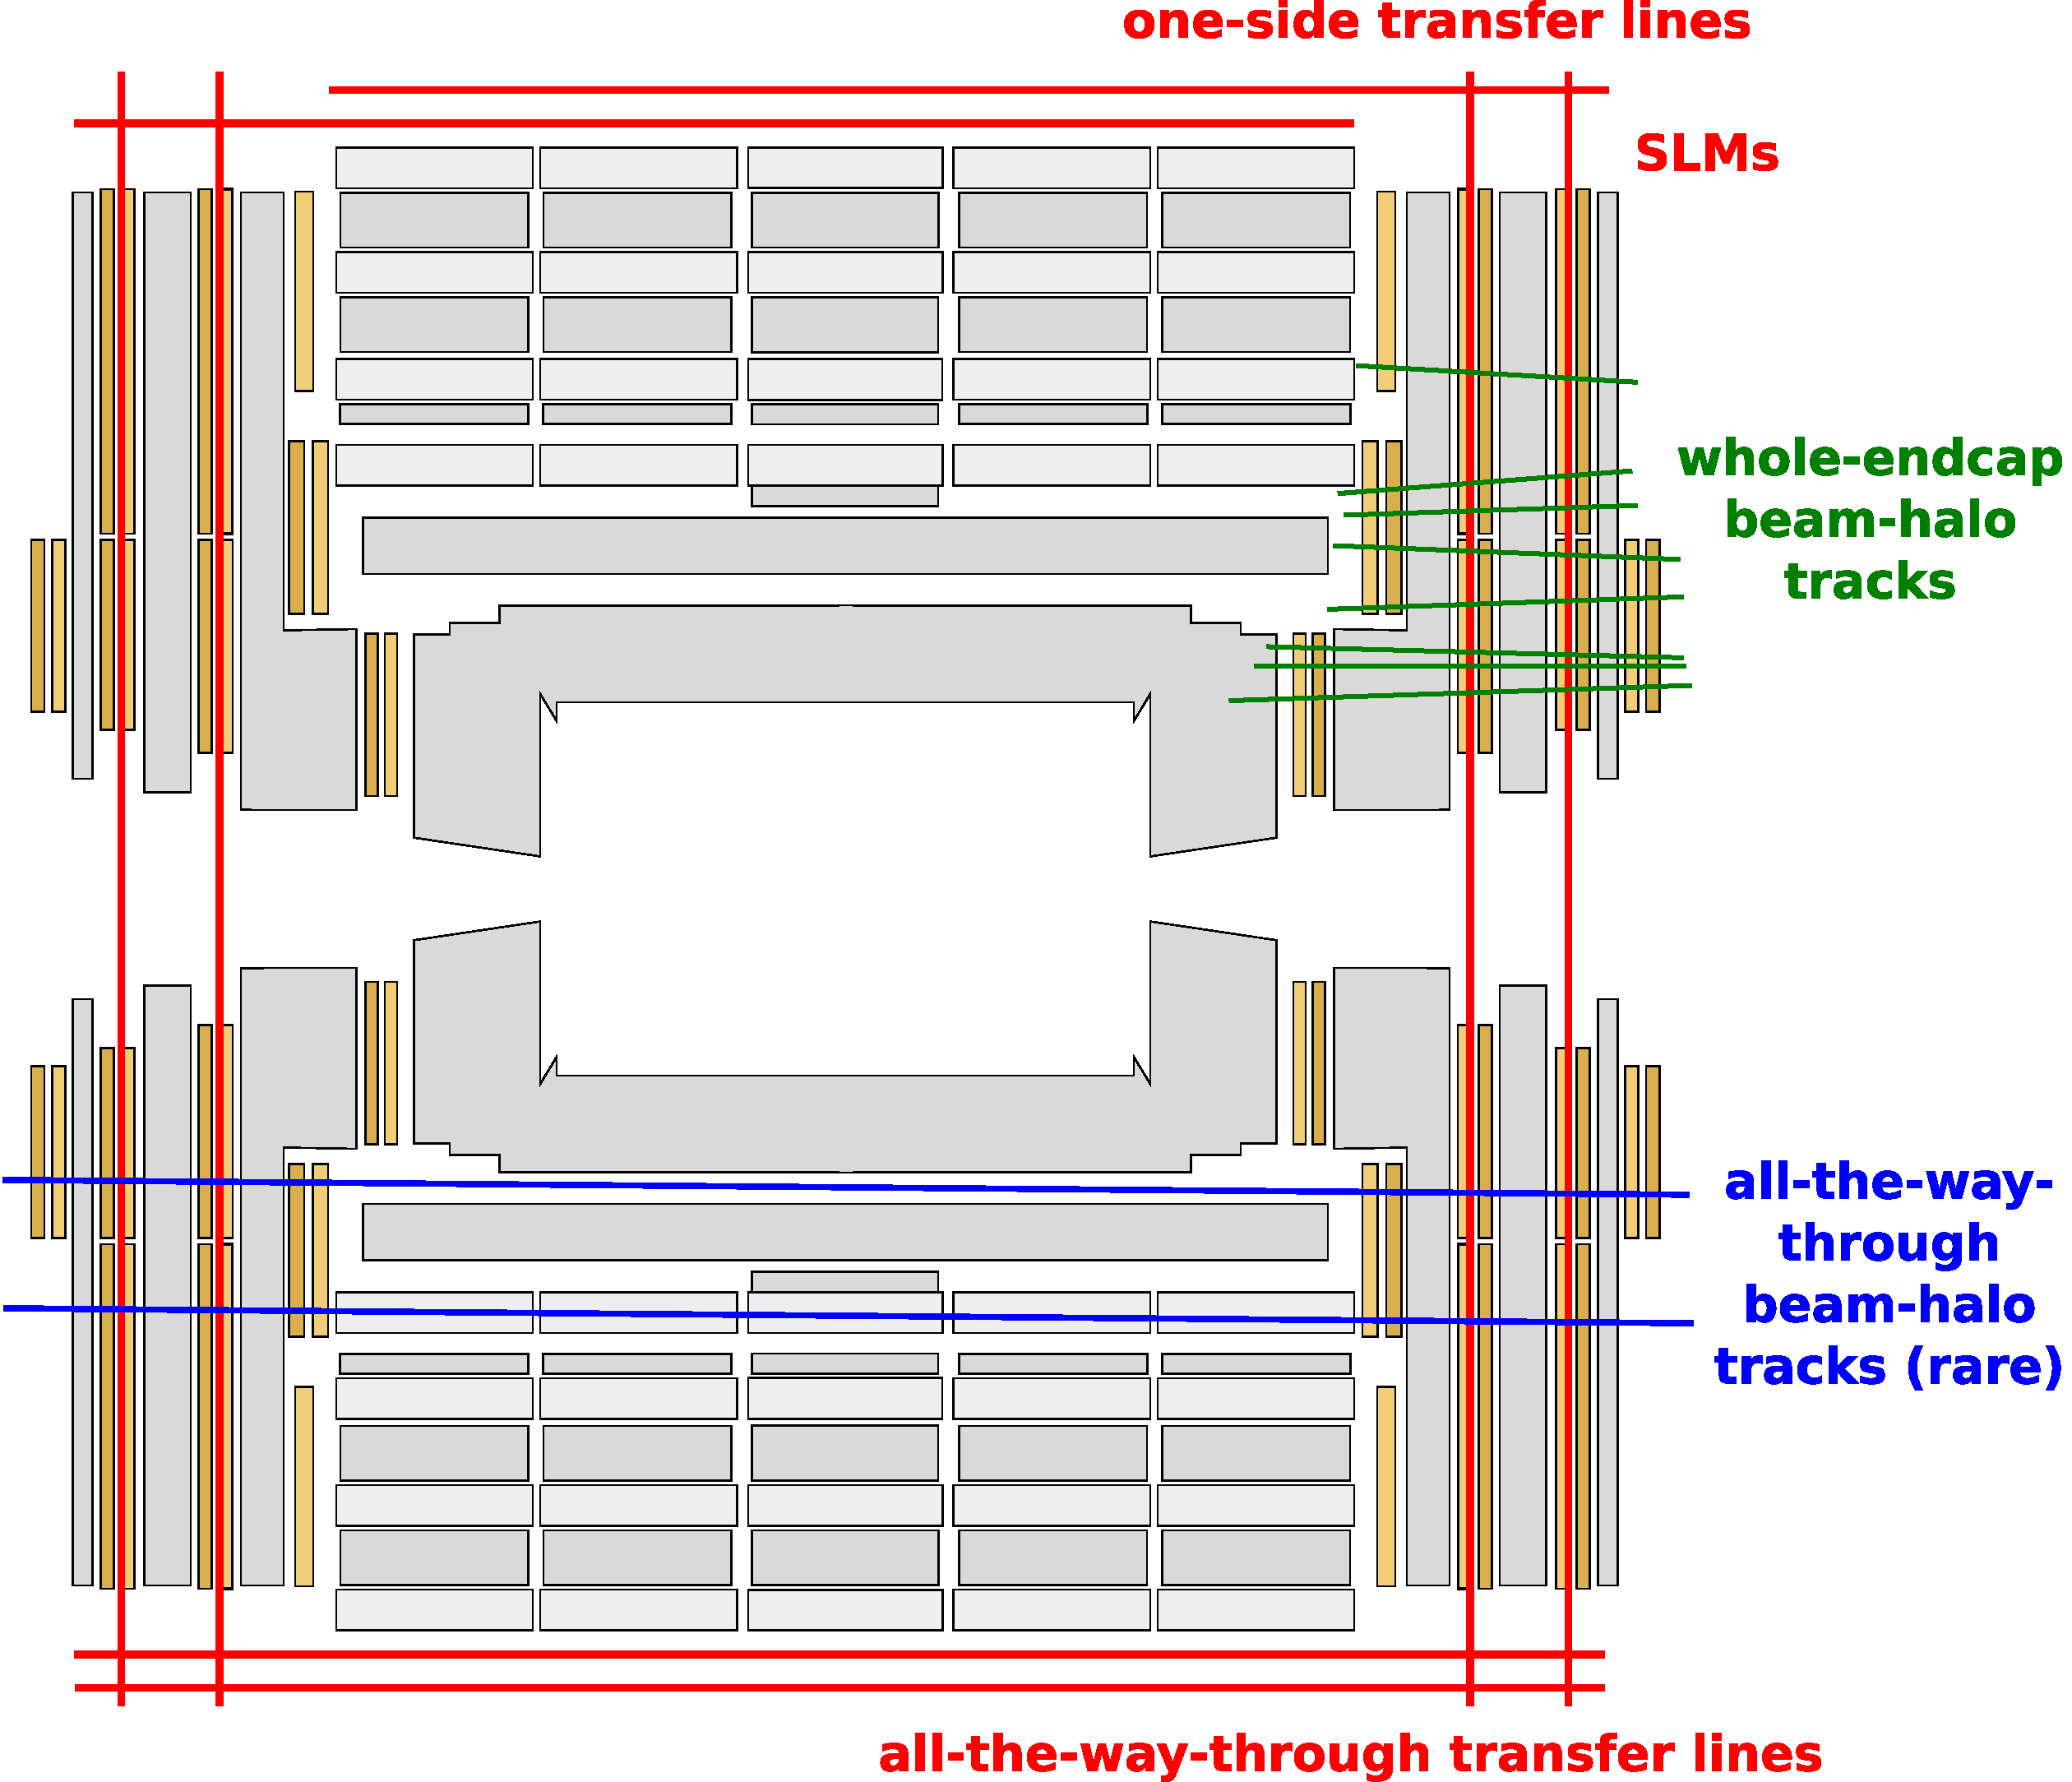
\includegraphics[width=0.9\linewidth]{beamhalo_transferlines.pdf}
\end{center}
\end{frame}

\begin{frame}
\frametitle{Idea \#2: beam-halo/transfer lines}

\vspace{0.2 cm}
\hfill 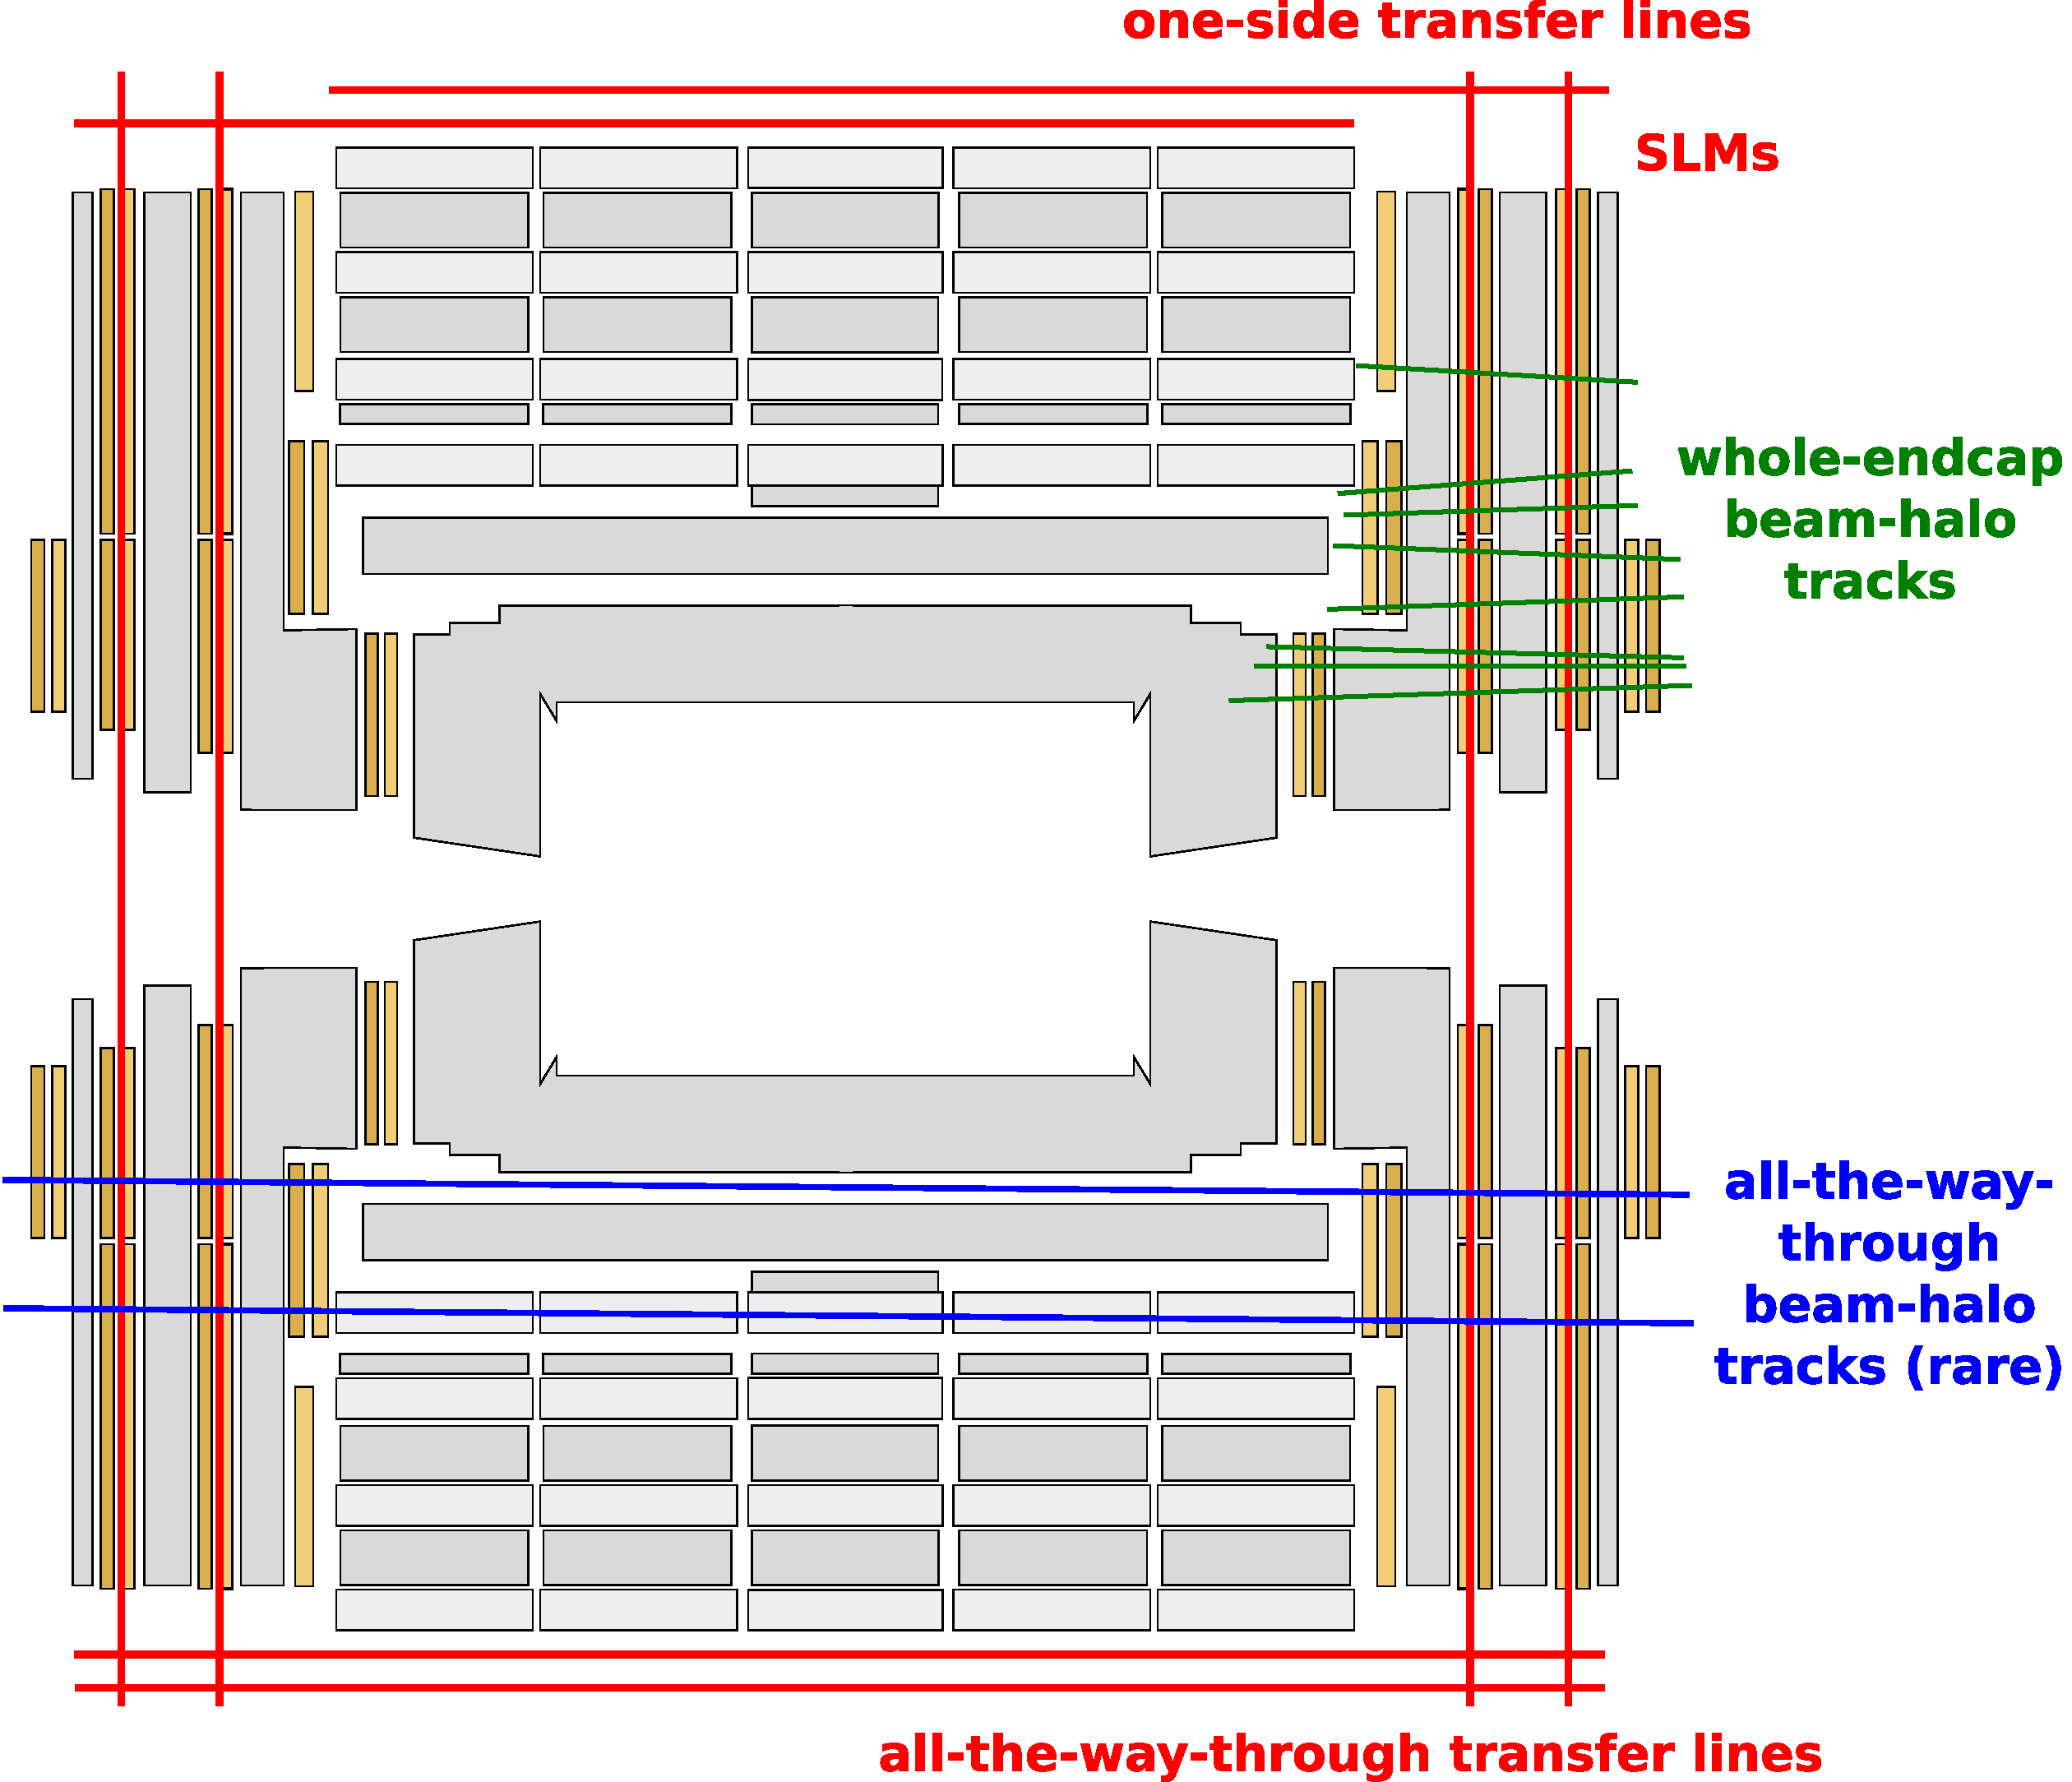
\includegraphics[width=0.4\linewidth]{beamhalo_transferlines.pdf}

\vspace{-4 cm}
\begin{itemize}
\item Beam-halo overlaps $+$ photo- \\ grammetry define well-aligned disks

\item \textcolor{darkgreen}{Whole-endcap beam-halo} aligns disks \\ relative to one another
\begin{itemize}
\item cross-check: are these disk \\ positions consistent with \\ GlobalMuons from tracker?
\end{itemize}

\item \textcolor{red}{SLMs} take chamber measurements \\ to transfer plates (cross-check: consistent with straight lines?)

\item \textcolor{red}{Transfer lines} take transfer plates to barrel
\begin{itemize}
\item cross-check: are the transfer line/MAB residuals straight lines?
\item \textcolor{darkblue}{barrel twist check: are those residuals sloped in $r\phi$ vs.\ $z$?}
\end{itemize}

\item All-the-way-through beam-halo can cross-check all-the-way-through transfer lines if both are available
\end{itemize}

%% \begin{minipage}{\linewidth}
%% \tiny No fitting is required: tracks provide a baseline alignment and
%%   coordinate frame: only need to check residuals (consistency) of SLMs
%%   and transfer lines with this baseline
%% \end{minipage}
\end{frame}

\begin{frame}
\frametitle{Pattern of cross-checks}

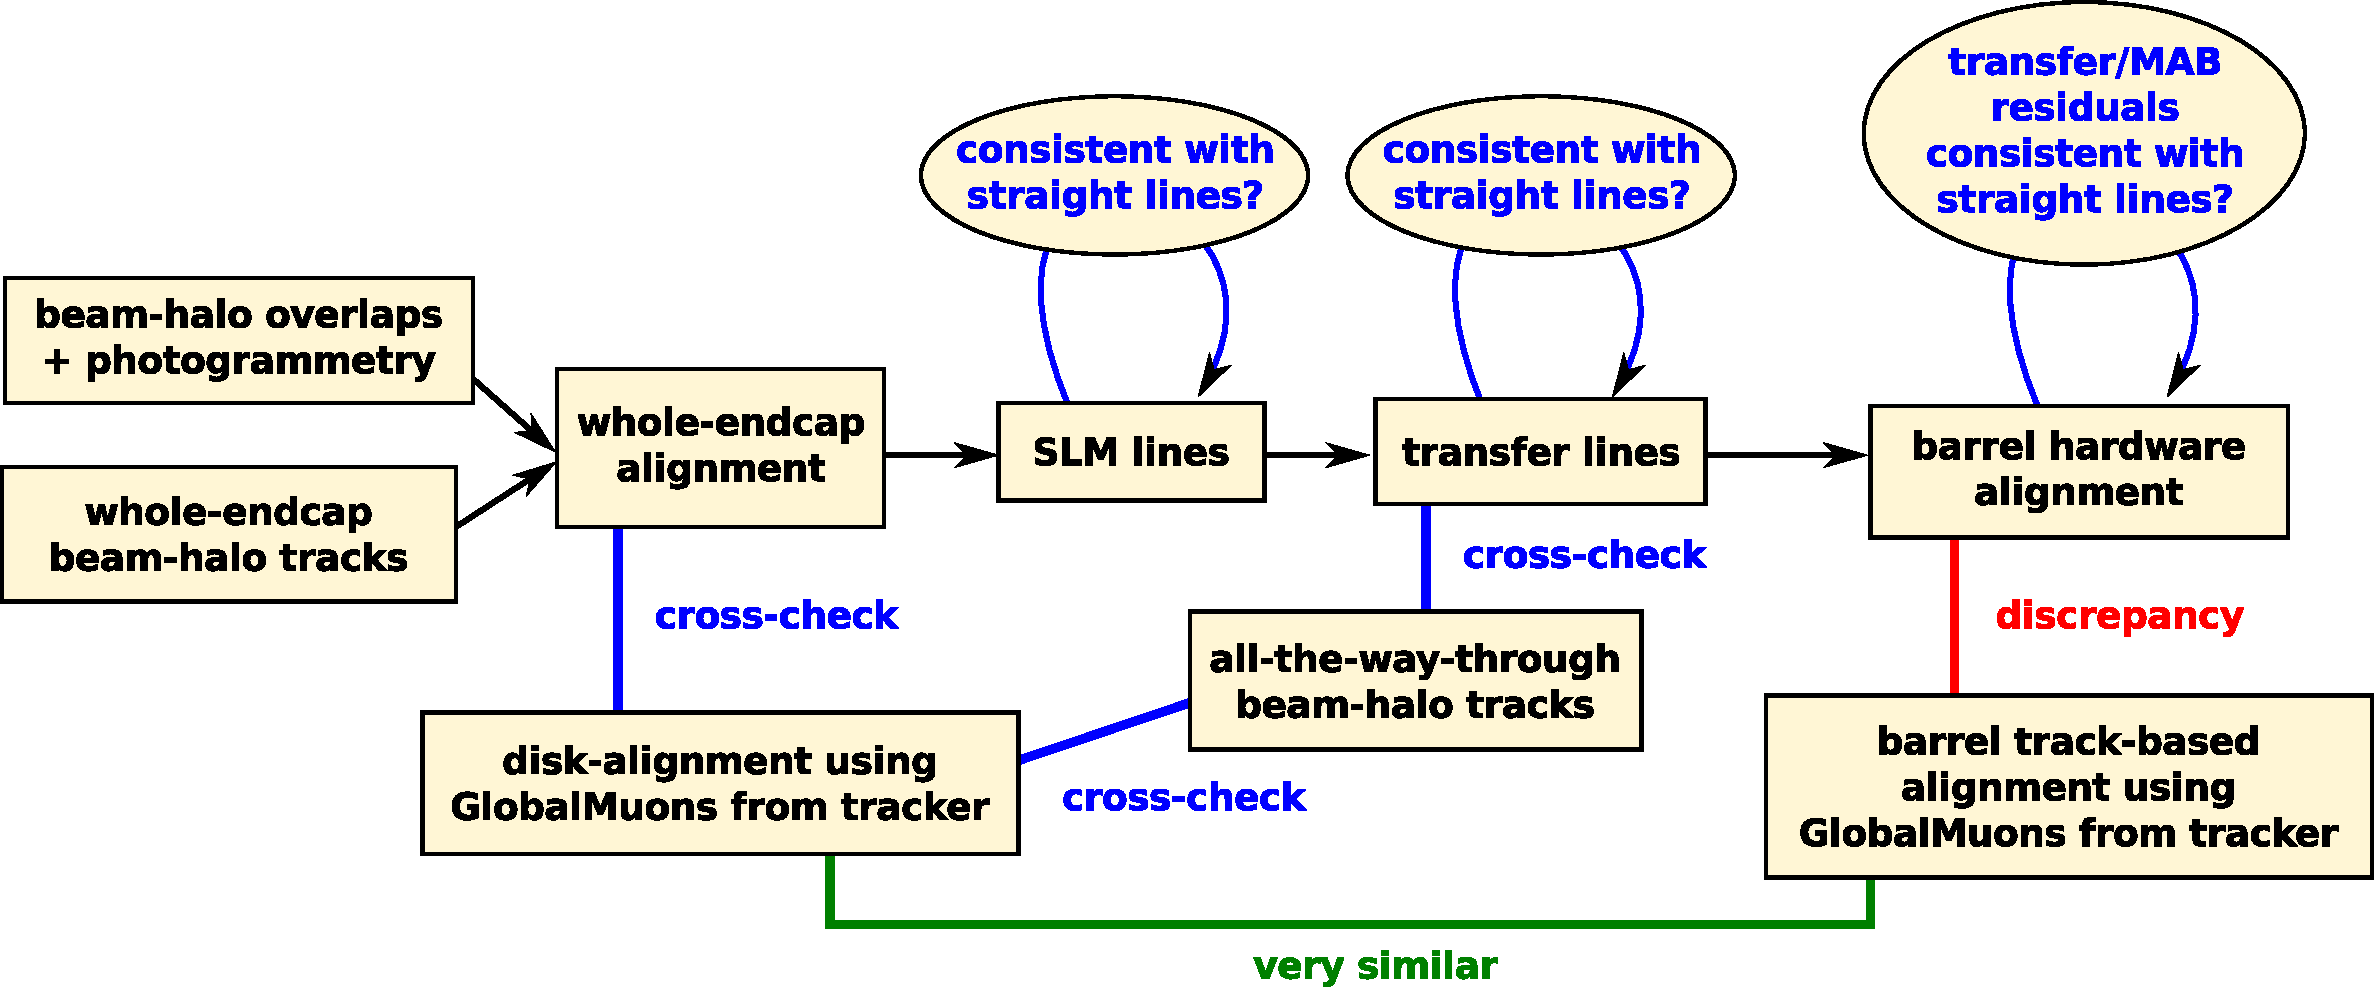
\includegraphics[width=\linewidth]{together.pdf}

\begin{itemize}
\item Doesn't require a separate hardware fit: just put hardware
  components in the geometry provided by track-based ``whole-endcap
  alignment'' and ask if hardware measurement residuals are consistent
  with straight lines
\item If any of the three ``straight-line consistency'' checks fail,
  then the barrel twist check is inconclusive (but we'll learn
  something about SLM/transfer lines)
\end{itemize}
\end{frame}

%% \section*{First section}
%% \begin{frame}
%% \begin{center}
%% \Huge \textcolor{blue}{First section}
%% \end{center}
%% \end{frame}

\begin{frame}
\frametitle{Conclusions}
\begin{itemize}\setlength{\itemsep}{0.3 cm}
\item If we can do this in the next two weeks, then we may get a
  compelling answer to the question of which barrel alignment to use

\item All of these cross-checks {\it pin-point} the system in which
  there may be a problem, and there's one track-based check in the
  middle of the hardware propagation chain

\item It improves our chances of knowing what's wrong, not just
  knowing that there's a problem somewhere
\end{itemize}
\label{numpages}
\end{frame}

\end{document}
